\documentclass[10pt,a4paper]{article}

% images
\usepackage[margin=1in]{geometry}
\usepackage{graphicx}
\usepackage{subfig}

\usepackage[title]{appendix}
\usepackage{pgfgantt}

% reference items
\usepackage{enumitem}

% links
\usepackage{url}
\usepackage{hyperref}

\usepackage{pdfpages}
\usepackage{pgfplots}

\usepackage{tikz}
\usetikzlibrary{arrows,automata,positioning}

\usepackage{footnote}

% maths
\usepackage{amsmath}
\usepackage{amssymb}
\usepackage{dsfont}
\usepackage{bm}

\usepackage{amsthm}

\theoremstyle{plain}
\newtheorem{theorem}{Theorem}[section]
\newtheorem{claim}[theorem]{Claim}
\newtheorem{lemma}[theorem]{Lemma}

\theoremstyle{definition}
\newtheorem{definition}[theorem]{Definition}

\newenvironment{subproof}[1][\proofname]{%
  \renewcommand{\qedsymbol}{$\blacksquare$}%
  \begin{proof}[#1]%
}{%
  \end{proof}%
}

\newtheorem*{claim*}{Claim}
\newtheorem*{corollary}{Corollary}
\newtheorem*{remark}{Remark}
\newtheorem*{fact}{Fact}

\DeclareMathOperator*{\argmax}{arg\,max}
\DeclareMathOperator*{\argmin}{arg\,min}
 
\newcommand{\code}[1]{\texttt{#1}}
\newcommand*\conj[1]{\overline{#1}}
\newcommand*\vect[1]{\bm{#1}}

% No section numbering
% \setcounter{secnumdepth}{0}

\bibliographystyle{siam}

\begin{document}

\begin{titlepage}
    \begin{center}

        \vspace*{2cm}
        
\includegraphics[width=.25\textwidth]{crest.png}

        \vspace*{1cm}
		{\Large \textsc{CS908 Assignment 4 - Dissertation specification}}

        \vspace*{1cm}
        \textbf{Thomas Archbold} \\
        1602581 \\
        Department of Computer Science \\
        University of Warwick \\~\\

        February 20, 2020 \\~\\

        \vfill

    \end{center}
\end{titlepage}

% Introduction (Background, Aims, Problem Statement)
% Related Work (Academic Research, Existing Systems)
% Research Processes (Approach, Methodology)
% Project Management (Timeline, Constraints, Risk)
% Progress
% Conclusion

% Problem definition and literature review        /20
% Research methodology and viability              /40
% Project plan: time management and risk analysis /10
% Communication skills                            /30

\section{Introduction}

	Prediction markets are exchange-traded markets\footnote{A market in which
	all transactions are routed through a central source.} that trade on the
	outcome of events rather than traditional financial instruments. Since
	actors in the market participate by putting up their own money in the form
	of betting on an unknown future outcome, the market prices can indicate the
	beliefs held by the market of certain events occurring. What can make these
	markets even more interesting is the ability to combine these bets in
	complex ways, giving users the freedom to make predictions over a range of
	different unknown outcomes. This is the approach taken by the combinatorial
	prediction market \emph{Predictalot}~\cite{Predictalot}, which provides a
	platform on which one can make bets on over 9.2 quintillion outcomes in the
	NCAA Men's College Basketball playoffs. This specification outlines the
	plans to implement a similar combinatorial prediction market for betting on
	outcomes in the 2020 United States presidential election, with a focus on
	implementing efficient ways for agents to interact with the market as well
	as methods to combine different collections of bets.

	The rest of the specification is structured as follows. In
	Section~\ref{sec:overview} we outline in greater detail the motivation for
	such a project and present our specific goals for the platform. In
	Section~\ref{sec:background} we discuss the underlying theory on which we
	will model the market, including relevant recent results in mechanism
	design for combinatorial auctions. We also discuss the current software
	that exists which implement other prediction markets, as well
	as how this project will fit in with the current body of work. In
	Section~\ref{sec:researchProcesses} we outline the methods and approaches
	we plan to take in order to complete this project, including a brief
	discussion of the tools, technology, and data that we expect to use. Aspects
	related to the effective management of the project are discussed in
	Section~\ref{sec:projectManagement}. We conclude with a brief discussion of
	progress made thus far in Section~\ref{sec:progress}, followed by closing
	thoughts and plans for the next stages in Section~\ref{sec:conclusion}.

\section{Project overview}
	\label{sec:overview}

	\subsection{Problem Statement}

	The goal of this project is to produce a combinatorial prediction market
	for the upcoming 2020 US presidential election on 3rd November and for
	related events in the run up to it. Participants within this market will be
	able to place and trade bets based on what they think is likely to happen,
	and these bets may be traded among users up until the outcome of the event itself is
	realised. Throughout this time, the platform will update the odds
	accordingly, taking into account the bets that have been made on related
	events. Winnings will then be paid out to those who own the bet.

	The project will be implemented as a web application written in Lisp, and
	in particular the Common Lisp dialect. The platform will allow for
	different auction mechanisms from the literature to be implemented and
	explored, with the secondary aim of measuring the impact of the underlying
	model on the market's functionality and performance.

	\subsection{Motivation}

	Prediction markets provide ways in which to bet on the occurrence of events
	in the future, and are often used to bet on a variety of circumstances --
	this could be on the outcomes of a political election, sporting events, or
	any other probabilistic event. Since there is an incentive to do well in
	such a market, as players stake their own money, people are inclined to bet
	how they truly feel about certain events, and hence the learning of public
	sentiment on these events can effectively be crowdsourced. Already this
	provides an exciting avenue to learn of public knowledge and belief on
	certain events. Combinatorial prediction markets, taking inspiration from
	the theoretical economics and mechanism design literature, allows for bets
	to be bought, sold, and combined in various ways and in doing so we may
	learn how the people view the likelihood of related and unrelated events.
	With this project, we seek to implement a combinatorial prediction market
	for events in the run up to the 2020 US presidential election, as well as
	the election itself, since there is significant global importance to these
	outcomes.

	From the mechanism design literature it is well-known that computing
	allocations of goods to buyers, as in a combinatorial exchange, that
	maximises, for example, social welfare or revenue, requires solving an
	NP-hard optimisation problem \cite{VCGNPhard}. Furthermore, for a market
	offering bets on $m$ separate events, there are $2^m$ possible ways of
	combining such bets -- how can we expect users to enter an exponential
	number of bids before they even get any items? These two problems are the
	focus of much of the literature within algorithmic mechanism design
	\cite{Nisan2001}, a subfield within algorithmic game theory at the
	intersection of economics and computer science that is concerned with
	designing the ways in which self-interested agents act within a strategic
	environment. They aim to achieve certain economic properties --
	truthfulness, budget balance, individual rationality, for example -- while
	ensuring that the mechanisms are practical to implement. It hence makes
	extensive use of techniques found in theoretical computer science, most
	notably asymptotic analysis, randomisation, and approximation. The goal is
	therefore to compute a solution that is approximately-optimal, or ``good
	enough'', rather than an optimal one that is infeasible to compute. With
	this in mind we wish to explore the challenges associated with implementing
	such a market.

	Even restricting ourselves to approximately-optimal solutions, however, we
	are faced with yet another problem -- how do we define ``good enough''?
	What makes, say, a 4-approximation for computing an allocation in a
	two-sided market any better than a 7-approximation that also achieves
	group-strategy proofness?\footnote{These are just examples to illustrate
	the point -- mechanisms with these guarantees may or may not exist.} The
	answer is that it depends -- trade offs must be made on a variety of
	assumptions on the structure of the market and its agents, and these
	parameters may be tweaked depending on the setting. Each of these decisions
	will lead to different mechanisms with different performance. Given that
	there is no single metric by which we can judge a mechanism's performance,
	this project also aims to implement software that allows for the tweaking
	of such parameters on the market to see what, if any, impact they have on
	the system as a whole. Thus the project can serve as a platform to
	implement and analyse recent mechanisms in the literature in a practical
	environment.

	We will give a brief justification for the choice of using the Lisp
	programming language, and in particular the Common Lisp dialect, to
	implement the project; the reasons are three-fold. Firstly, since the
	project involves creating a web application we will need to use a language
	for which there are sufficient libraries to do so: Quicklisp
	\cite{Quicklisp} is a library manager for Common Lisp that provides an
	extensive selection of libraries and is compatible with many Common Lisp
	implementations. In particular, we have several options available to us for
	writing a dynamic and responsive web application. The specific libraries we
	expect to use are detailed in Section \ref{sec:researchProcesses}.
	Secondly, Lisp is an expressive high-level programming language that Peter
	Seibel claims ``... will get a lot done with code that simply and clearly
	expresses your intention'' \cite{PracticalCommonLisp}. This certainly does
	much to sell it. Unique to Lisp is the Read-Evaluate-Print-Loop (REPL), and
	effective use of this allows for quick and dynamic implementation and
	testing. Changes may even be made while a Lisp program is executing, which
	can streamline the development process. Finally, Lisp nowadays seems a
	somewhat unconventional choice of language, and would be intriguing to use
	in a practical setting, even if just to build on the limited experience
	with it so far.

	\subsection{Aims}

	As stated, the main aim of this project is to create a combinatorial
	prediction market for betting on outcomes in the forthcoming US
	presidential election. The underlying exchange will be modelled as variants
	of two-sided combinatorial markets (see Section~\ref{sec:background} for a
	more in-depth discussion of what this entails). We detail the features of
	the project below under the categories of \textbf{core},
	\textbf{additional}, and \textbf{stretch} features. The core features will
	implement all of the functionality to qualify the software as a
	combinatorial prediction market, and will cover making and buying basic
	bets, combining them in complex ways, and calculating the somewhat accurate
	based on the actions of the market, likely based on dummy data for testing;
	the additional features will extend this functionality so we may begin to
	explore the effects of making use of different underlying mechanisms from
	the literature; and the stretch features will focus on transitioning from
	the dummy data into the real world, as well as the provision of more
	complex bets and further refinement of the user experience.

	\subsubsection{Core features}

	The project will have:

	\begin{itemize}
		\itemsep0em
		\item A web application written in Common Lisp on which to host a
			combinatorial prediction market for the run up to the US
			presidential election, modelled as a two-sided combinatorial
			auction

		\item The ability for multiple users to interact within this market,
			and specifically:
			\begin{itemize}
				\itemsep0em
				\item Propose bets on a number of events
				\item Buy bundles of bets from other users, transferring the
					right to the winnings should the outcome be realised
				\item Compute approximately-accurate odds based on the trades
					which take place, and distribute winnings accordingly
			\end{itemize}

		\item The ability for users to make bets on the outcomes of the
			following events:
			\begin{itemize}
				\itemsep0em
				\item the 2020 presidential winner
				\item the party that wins the presidency
				\item each state's Democratic primary elections
				\item each state's Republican primary elections
				\item the Democratic nominee
				\item the Republican nominee
			\end{itemize}

		\item A database for persistent storage of user information

		\item The web application run on dummy data, so that the market
			mechanisms may be tested for correctness

		\item The ability to react asynchronously to user input
	\end{itemize}

	\subsubsection{Additional features}

	The project should have:

	\begin{itemize}
		\itemsep0em
		\item Functionality to collect real-world data, moving the application
			away from simulation and into reality

		\item Various ways in which users may interact in trades, including
			the traditional method of selecting a single item, as well as
			assuming single- and $k$-minded bidders

		\item Implementations of various two-sided market mechanisms from the
			literature, including deferred acceptance auctions

		\item The provision for more complex types of bets
	\end{itemize}

	\subsubsection{Stretch features}

	The project may:

	\begin{itemize}
		\itemsep0em
		\item Be extended to other domains, such as sports tournaments or other
			political campaigns

		\item Take additional aesthetic and usability considerations
	\end{itemize}

\section{Background}
	\label{sec:background}

	\subsection{Combinatorial auctions}

	In a single-item auction, we have a collection of $n$ agents who each
	possess a valuation for acquiring a single item on offer. A
	\emph{mechanism} is any method for allocating this item to the bidders:
	typically, this involves specifying an \emph{allocation rule} and a
	\emph{payment rule}. The former may be responsible for collecting
	information from the participants -- often a bid -- to compute the
	allocation, while the latter is used to ensure that agents act truthfully.

	The real number $v_i$ denotes agent $i$'s valuation for acquiring the item.
	This information is private to each agent (referred to as ``bidders'' or
	``buyers''), meaning neither the mechanism nor the other agents know this
	value. Naturally, we wish to allocate this item to the bidder who truly
	values it the most -- that is, allocate it to agent $i^* = \argmax_{i \in
	[n]} v_i$.\footnote{The standard notation of $[k]$ is used to represent the
	set $\{ 1, \ldots, k \}$} It is a typical for an auction to elicit a bid
	$b_i$ from each agent so as to acquire their valuation $v_i$ -- note,
	however, that since the agents are strategic they may lie (i.e., submit bid
	$b_i \neq v_i$) if they believe it is in their best interests. The Vickrey
	mechanism \cite{Vickrey1961} achieves such an optimal allocation by
	``believing'' the bidders, giving the item to the agent with the highest
	bid, and charging him the next highest bid.

	This can be extended to the case of multi-item auctions, in which we have
	$m$ items to allocate. Buyers now have a collection of valuation function,
	$v_i(S)$ that associate to each subset of items $S \subseteq [m]$ a value
	for acquiring this subset. However, since the number of subsets of any set
	of size $m$ is $2^m$, we cannot hope to either collect all these valuations
	from bidders nor use them in sub-exponential time, unless we impose some
	restrictions. In the literature, one common way to deal with this obstacle
	is by restricting the bidders to be $k$-minded -- each bidder submits a
	maximum of $k$ bids for $k$ different subsets, and effectively a bid of
	zero for every other set. There are also subtleties involved in allowing
	items to be homogeneous, in which case the auction contains $m$ copies of
	the same item, or heterogeneous, where each item is unique. The idea of
	this project is to model bets on future outcomes as items, and since we
	will be combining different bets to learn about public sentiment on these
	outcomes, we assume the items in the auction to be heterogeneous.
	Furthermore, since we are keen to explore the practical performance of some
	of the mechanisms in the literature, we will often use the $k$-minded
	bidders model in our underlying representation of the auction mechanism.

	In a combinatorial auction, instead of simply maximising over $n$ numbers
	as in a single-item setting, i.e. selecting the single bidder with the
	highest bid, we must maximise over all possible allocations. In this
	setting, we aim to maximise social welfare, or the sum of the agents'
	valuations. If a mechanism computes allocation $A = (A_1, \ldots, A_n)$,
	where agent $i$ is allocated subset $A_i$, then the value we are maximising
	as a function of this allocation is $W(A) = \sum_{i \in [n]} v_i(A_i)$. The
	analogue to the Vickrey auction in the multi-item setting, the
	Vickrey-Clarke-Groves mechanism \cite{Vickrey1961, Clarke1971, Groves1973},
	again believes the bidders, awarding items to agents who value them most
	and charging each bidder their \emph{externality}, or the extra cost in
	social welfare incurred by that agent participating in the auction.

	Until now we have assumed that the auction itself holds the items --
	this will not be the case in our prediction market since the agents will
	propose and hold the bets. It is therefore useful to have the concept of a
	\emph{two-sided} market. This comprises a set of two distinct types of
	agents: sellers, who initially hold the items for sale, and buyers, who are
	interested in buying the items from the sellers. Using the model of
	Colini-Baldeschi et al.~\cite{ColiniBaldeschi2017}, formally a two-sided
	market is a tuple $(n, m, k, I, G, F)$, where $[n]$ is the set of buyers,
	$[m]$ is the set of sellers, $[k]$ is the set of items, and $I = (I_1,
	\ldots, I_m)$ is the \emph{initial endowment}, such that $I_j$ is the set
	of items initially held by seller $j$. Vectors $G = (G_1, \ldots, G_n)$ and
	$F = (F_1, \ldots, F_m)$ are the distributions from which the buyers' are
	sellers' valuation functions are assumed to be drawn, respectively. The
	notion of an allocation changes only slightly under this model: given a
	two-sided market, our aim is to redistribute the items among the agents so
	as to maximise the social welfare. An allocation is hence a pair of vectors
	$(X,Y) = ((X_1, \ldots, X_n), (Y_1, \ldots, Y_m))$ such that the union of
	$X$ and $Y$ is the set of items $[k]$, and $X_1, \ldots, X_n, Y_1, \ldots,
	Y_m$ are mutually disjoint, meaning no two agents are allocated the same
	item. As before, buyers have a valuation $v_i(S)$ for each subset of items
	$S$; we have a similar concept for the sellers,	denoted $w_j(S)$. The goal
	is still to maximise the social welfare, which is now:

	\begin{equation*}
		W(X, Y) = \sum_{i \in [n]} v_i(X_i) + \sum_{j \in [m]} w_j(Y_j)
	\end{equation*}

	We conclude our discussion of the underlying model by introducing some of
	the desirable economic properties of the mechanisms, useful in our
	discussion of the current literature:

	\begin{itemize}
		\itemsep0em
		\item \textbf{Incentive Compatibility (IC):} agents are incentivised to
			bid truthfully (i.e. submitting $b_i = v_i$) as they can do no
			better by lying -- truth-telling is a \emph{dominant strategy}.

		\item \textbf{Individual Rationality (IR):} it is not harmful for any
			agent to participate in the market, meaning in any trade there is a
			strategy that yields a utility that is no less than their initial
			utility. Note that this says nothing about the outcome of the event
			-- agents may still experience a net loss for having purchased a
			bet which turned out to be false.

		\item \textbf{Budget Balance (BB):} the sum of all payments is at least
			zero, meaning no extra funds have to be supplied to subsidise the
			market.

	\end{itemize}

	\subsection{Related work - auctions}

	Algorithmic mechanism design enjoys much attention in the setting of
	combinatorial auctions, where there is ample opportunity to make use of
	techniques from theoretical computer science. Much of this is inspired by a
	question posed shortly after the field's inception by Nisan and
	Ronen~\cite{Nisan2001}, which asks whether the requirement for dominant
	strategy incentive compatibility inherently degrades a mechanism's
	approximation ratio -- put another way, it asks if mechanism design is
	inherently harder than algorithm design. This question is answered in part
	by Daniely, Schapira, and Shahaf~\cite{Daniely2018}, who present various
	inapproximability results for deterministic, truthful mechanisms.

	To sidestep the obstacles faced by deterministic mechanisms,
	Colini-Baldeschi et al.~\cite{ColiniBaldeschi2017} make use of
	randomisation to present three constant-factor approximation mechanisms for
	two-sided combinatorial markets, under various assumptions about agent
	valuations. In particular, they provide three 6-approximation mechanisms
	which achieve individual rationality, incentive compatibility, and a
	stronger notion of budget balance, termed Direct Trade Strong Budget
	Balance (DSBB). Two-sided combinatorial auctions are also considered for
	single-minded bidders by D\"utting, Gkatzelis, and
	Roughgarden~\cite{Dutting2017}, in which they study Deferred Acceptance
	(DA) auctions. These auctions compute an allocation by repeatedly rejecting
	the least promising candidate in a greedy manner, in this case the lowest
	bid. DA auctions have preferable incentive guarantees over simple VCG or
	greedy mechanisms in that they are (weakly) group strategy proof, meaning
	there is no way for a coalition to act such that each member of the
	coalition is better off. They introduce a polynomial-time mechanism that
	achieves the incentive-compatibility of a DA auction and a $O(\log
	m)$-approximation. In a similar vein to Daniely et al.~\cite{Daniely2018},
	they prove inapproximability results for DA auctions in the setting of
	single-minded bidders; specifically, that they cannot achieve a better
	approximation ratio than $o(m)$ if the way in which the mechanism ranks
	bids is of a particular form.

	Dughmi, Roughgarden, and Yan~\cite{Dughmi2016} use randomisation to provide
	a mechanism that is truthful in expectation and achieves a constant factor
	approximation of $O(1-1/e)$ for welfare maximisation with heterogeneous
	items. They show that this is a polynomial-time mechanism in expectation,
	further proving that the approximation ratio is the best possible assuming
	P $\neq$ NP. Dobzinski and Nisan~\cite{Dobzinski2010} make use of
	Maximal-In-Range and Maximal-In-Distributional-Range~\cite{Dobzinski2006}
	mechanisms to introduce several DSIC approximation mechanisms for computing
	multi-unit auctions in polynomial time. These are mechanisms which search
	over a pre-specified range for a maximal solution. They present a
	2-approximation for general valuation functions, and a Polynomial Time
	Approximation Scheme (PTAS) for bidders with $k$-minded valuations.
	Although this assumes there are multiple copies of items, and hence likely
	unsuitable to our setting, it would be interesting to explore the use of
	such a framework.

	\subsection{Related work - prediction markets}

	In the literature, prediction markets have been used in a variety of ways
	to predict the outcomes of a range of events, such as in business and
	politics \cite{Spann2003, Berg2006}. Their power is shown by Nay, Van der
	Linden, and Gilligan~\cite{Nay2016} who analyse prediction markets
	empirically to study the how the factors describing the market affect the
	agents' beliefs on the real-world outcome. They make the argument for a
	prediction market for betting on the cause of global warming, either
	through CO$_2$ emissions or through variations in solar intensity, and show
	that increased agent participation causes public feeling to shift towards
	the ``true'' climate change model. Thus they suggest that a climate
	prediction market would be useful for generating broad consensus on the
	causes of climate change.

	In order for these markets to function, they require a central trusted
	entity to verify the true outcome of the event, however Freeman, Lahaie,
	and Pennock~\cite{Freeman2017} identify this as a bottleneck of what can be
	predicted, motivating their study of decentralised prediction markets. This
	allows for the outcome to be determined by a group of arbiters who may
	themselves be participating, i.e. holding a stake, in the market. Given
	the greater incentive these agents may have to sabotage the mechanism, they
	derive mechanisms under which they are incentivised to act truthfully.
	Peterson et al.~\cite{Peterson2015} also study this setting in their paper
	and use it to implement the decentralised oracle at the heart of their
	prediction market platform \emph{Augur}~\cite{Augur}.

	In the centralised setting, Kroer, Dud\'ik, Lahaie, and
	Balakrishnan~\cite{Kroer2016} present a combinatorial prediction market
	that makes use of a cost-based market maker, in which all bets are bought
	from and sold to the market maker, rather than the traders, which they
	argue can be desirable in combinatorial auctions due to the possibility of
	low liquidity. This is the case in which there are no sellers interested in
	trading with a buyer; in contrast, a market maker is always available to
	trade. Our platform will consider a smaller space of events compared to the
	NCAA Men's College Basketball playoffs however, hence our decision to use a
	more natural two-sided market to model the interactions between agents.

	\subsection{Existing systems}

	There are several examples of recent implementations of prediction markets
	in various settings. This project's conception was initially inspired by
	\emph{Predictalot} \cite{Predictalot}, a combinatorial prediction market
	for betting on the outcomes of a wide range of events in the NCAA Men's
	College basketball playoffs. It launched as a Yahoo! app in 2010, though it
	appears to have since been abandoned. Nonetheless, it boasts the ability
	to bet on ``almost anything you can think of, like \emph{Duke will advance
	further than UNC}''. Specifically, the tournament is structured such that
	the top 64 college basketball teams play 63 games in a single elimination
	tournament, while \emph{Predictalot} keeps track of the odds, computing
	them by scanning through all the predictions placed so far. They note that
	an exact computation of the odds is \#P-hard -- as hard as counting the
	number of variable assignments that satisfy a given CNF formula, or how
	many subsets of a list of integers sum to zero -- hence justifying their
	decision to approximate the odds by random sampling of the outcome space.
	They also emphasise that they keep track of all different possible
	outcomes, resulting in odds that are interconnected in natural ways --
	betting on a team to make the final will have an effect on the odds of each
	stage, since the team must win at each of these stages to reach the final
	in the first place. Given the apparent power behind this idea, it would be
	interesting to apply it to a setting with perhaps more significance, such
	as the upcoming presidential elections.

	As discussed, \emph{Augur} is more recent example, launching in 2018 on the
	Ethereum blockchain. Similarly to how this project will be structured,
	\emph{Augur} hosts the prediction market in two phases: the market stage,
	where users are able to trade shares between each other, and the
	arbitration stage, where the market's outcome is determined. However,
	\emph{Augur} makes use of fees to subsidise the arbitration process,
	breaking the budget balance property discussed earlier. This makes it less
	appealing, as money is required to be fed into the system in order for it
	to function.

	Both \emph{PredictIt} \cite{PredictIt} and the Iowa Electronic Markets
	(IEM) \cite{IEM} provide the ability to make bets on various political
	events, including on outcomes within the 2020 US presidential election.
	However, like \emph{Augur}, they do not provide the ability to combine
	these bets in complex ways and hence this is a gap that this project aims
	to fill.

	This project will differ from these mainly in the fact that we will
	implement a combinatorial prediction market, with a focus on making bets on
	a combination of outcomes -- the only similar existing software
	implementing this was \emph{Predictalot}, which is no longer maintained or
	even accessible. Betting on collections of events better incorporates
	conditional information into the market price, hence giving a more
	realistic view of how events are related. The project will also differ in
	the means by which users will interact with the markets. Specifically, on
	each of the existing systems discussed, the prices of bets are shown and it
	is up to the user if they wish to participate in the trade at that price.
	This project will model these interactions more akin to sealed-bid
	auctions, with the intention that bidders will place and buy bets that
	align more closely with their true beliefs. Placing such additional
	restrictions these interactions with the market allows for stronger
	performance guarantees and allows more easily for results from the current
	literature to be implemented. Of course, it will be an important design
	decision to trade off between achieving these guarantees while ensuring the
	platform feels natural to use.

	\begin{figure}[h]
		\centering
		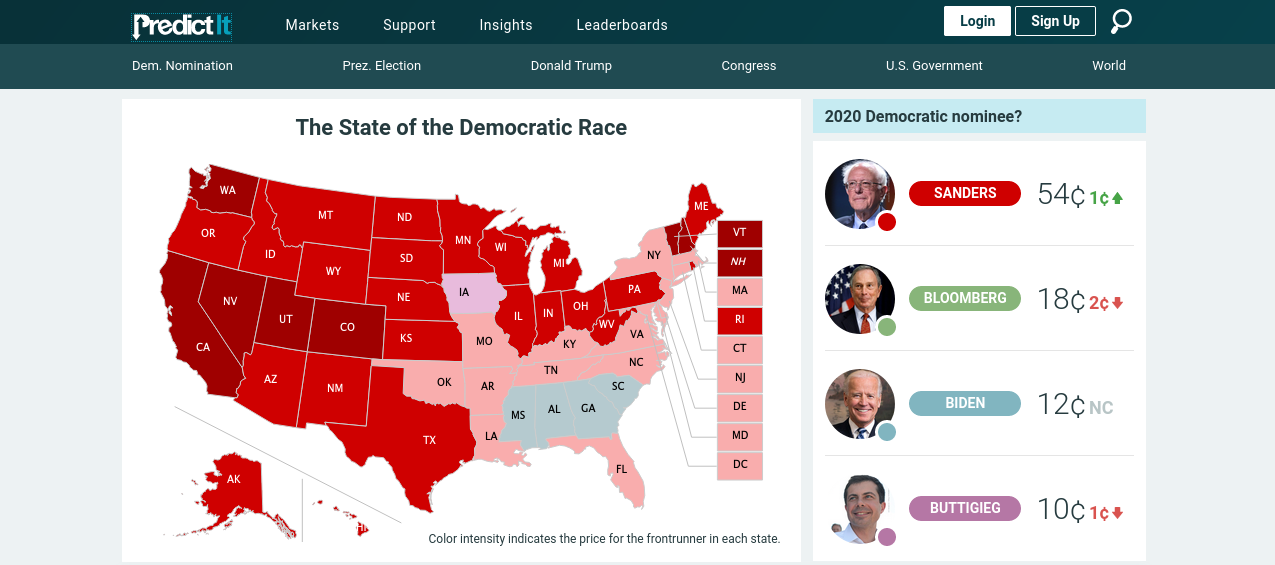
\includegraphics[width=.8\textwidth]{predictit.png}
		\caption{The \emph{PredictIt} prediction market for the 2020 Democratic
		nominee}
		\label{fig:predictit}
	\end{figure}

% Research Processes (Approach, Methodology)
\section{Research Processes}
	\label{sec:researchProcesses}

	\subsection{Approach}

	Although much reading has been done on papers in the literature on
	algorithmic mechanism design for combinatorial auctions, more will be done
	over the course of the project's completion to stay abreast of recent
	results and possible avenues for implementation. The body of research on
	two-sided markets is relatively extensive, and hence there should be no
	shortage of material to cover. More research needs to be done, however, on
	prediction markets in general in order to better understand how they
	function. Given that \emph{Augur} is open-source it is likely to prove a
	key source of information about implementing such markets -- more
	qualitative observations on how prediction markets work will also be
	gathered by getting familiar with the various existing systems out there,
	whose code is not open-source. The e-Print archive \emph{arXiv.org} will be
	a key tool for further exploring recent developments in prediction markets.

	\subsection{Tools} 

	As mentioned we will be implementing the project in Common Lisp. We plan to
	use the following libraries: CL-WHO \cite{CL-WHO}, for converting Lisp
	expressions into HTML; Hunchentoot \cite{Hunchentoot}, a web server written
	in Common Lisp and a toolkit for hosting dynamic websites; Parenscript
	\cite{Parenscript}, which will allow us to compile Lisp expressions into
	JavaScript, for client-side validation; and SmackJack \cite{SmackJack}, a
	small AJAX framework for Common Lisp which allows us to create asynchronous
	functionality in our web application. The REPL is a key tool available to
	Lisp, and we plan to make full use of it to quickly and dynamically
	implement changes. \LaTeX will be used for all written documentation, and
	most code is likely to be written in Vim.

	We plan to make extensive use of Git \cite{Git} by way of version control
	software -- previous experience dictates this as an essential aspect to our
	development pipeline. The project will be hosted on Github, meaning
	development can take place essentially from anywhere (and at least on
	computers with a Common Lisp implementation), and all the necessary files
	are stored where they are guaranteed not to be lost. Github also allows for
	the progress to be more easily tracked (an example is given in
	Fig~\ref{fig:commit_graph}). Progress can more easily be checked against
	the project timetable in this way, not only by viewing how many commits are
	being made, but also which features are being added each time. This will
	simplify the evaluation process for the interim report and final write-up,
	as one can see exactly what features are added and when.

	\begin{figure}[h]
		\centering
		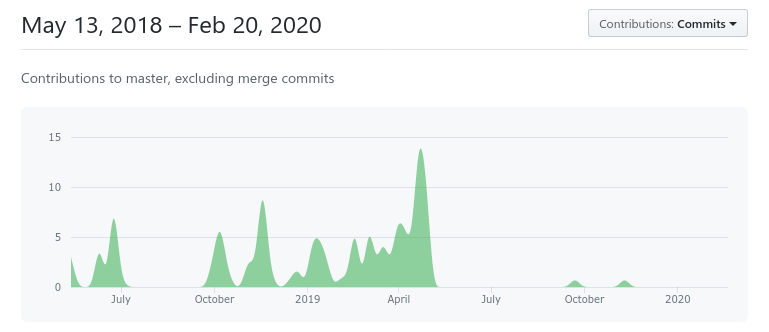
\includegraphics[width=.8\textwidth]{commits.png}
		\caption{Visualising commits in Github}
		\label{fig:commit_graph}
	\end{figure}
	
	To allow for multiple users to interact within the market the web server
	will eventually need to be hosted somewhere, as opposed to simply being run
	locally. A possible (free) tool for hosting the server is therefore Ngrok
	\cite{ngrok}, which provides the ability expose a local web server for
	public use. This will suffice for the small scale scope of this project,
	and can easily be hosted elsewhere should the need arise.

\section{Project Management}
	\label{sec:projectManagement}

	\subsection{Overview}

	Regarding the development of the software, we plan to mix between a
	plan-driven and agile approach. Initially there is a set order in which
	features are to be added, such as setting up the development environment,
	getting the web server up and running, and designing the systems that will
	store user information and allow for interactions between agents. Once the
	basics of the prediction market are implemented, the areas on which to
	spend development may open up, and hence focus may shift to an agile
	approach. Specifically, decisions will need to be made at the time on which
	features are most in need of attention. An initial outline of the timeline
	for the project is provided in Appendix~\ref{app:timetable}.

	On the administrative side, weekly meetings with project supervisor
	Dr Englert will be held in order to track and discuss progress regularly.
	Moreover, they provide the opportunity to bring up issues as they occur so
	that solutions may be discussed and attempted quickly. Meetings will take
	place on Tuesdays between 5pm and 6pm.

	\subsection{Constraints}

	Since the project will mostly be developed and tested locally, there are
	few external constraints that could hinder progress. Once the project
	begins to take fuller shape, it will be required to be tested using
	multiple (non-simulated) users, and there may be additional unforeseen
	difficulties in providing for this. Testing in this phase is likely to be
	done with informal quality assurance testing with colleagues. A risk
	associated with this is that they may be busy (perhaps testing their own
	dissertations), but this is unavoidable.

	There is little progress likely to be made during the exam period and the
	weeks leading into it as most attention will be towards revising. This is
	an acceptable constraint given the vacuum of activity over the summer that
	follows, which provides ample time to compensate for this deficit.

	\subsection{Ethical concerns}

	All development and initial testing will be done independently, hence there
	is no reliance on using external data from the outset. Once we integrate
	real-world data into the platform, all data we gather regarding the US
	election will all be public knowledge, meaning there is no ethical concern
	here. Since testing will be performed informally with the help of
	colleagues, there are no legal or professional issues to worry about in
	this regard, either.

	\subsection{Project Timeline}

	The rest of the term will be spent getting up to speed with the current
	literature surrounding prediction markets, in order to see how they have
	been implemented by others and what is considered state-of-the-art. Given
	the course load towards the end of this term from other modules, relatively
	less focus will be given towards this project. However, regular work will
	be done in setting up the necessary tools and environments so that the
	foundations for the prediction market itself to be implemented will be in
	place by the end of the term. This involves becoming better acquainted with
	Common Lisp; setting up the web server using Hunchentoot, and designing the
	database to store all the relevant data. Furthermore, it will involve
	implementing a basic two-sided combinatorial auction mechanism that acts on
	dummy data, again to build foundations for the work ahead.

	During the second half of the Easter break, most time will be dedicated to
	revising for exams, and this will last until the end of exams around
	mid-June. Work will still be done during this period, and should be simple
	to implement given that all necessary foundations have been put in place by
	this time. In particular, during this time we will be implementing the
	necessary computations for displaying accurate odds for bets, based on the
	trades that have taken place so far. Initially these odds will be
	calculated in a simple manner, that is, not in a way analogous
	to \emph{Predictalot}'s method. We will then write the system to pay
	winnings out to the appropriate agents.

	After the exam period we will work on refining the computation of the odds,
	so that a more accurate idea of public sentiment may be achieved by
	combining the bets made in complex ways. During this point we will also
	begin to experiment with implementing more advanced mechanisms from the
	literature, including a deferred acceptance auction. Since the project
	presentation will be delivered around this period, work will begin roughly
	a month prior to provide ample time to prepare.

	Throughout the summer we will begin to gather real-world data for the
	market and begin testing the application. Much of this time will be spent
	writing up the final report; we aim to finish a draft of this well in
	advance of the 10th September deadline, to give time to gather and
	implement feedback. The main bulk of the software will need to be done by
	the beginning of August, and the first draft on the report done by
	mid-August.

\section{Progress}
	\label{sec:progress}

	\subsection{Current progress}

	Some progress has been made thus far with regards to implementing the
	project. The development environment is currently being set up, which
	includes downloading the aforementioned packages from using Quicklisp and
	ensuring they run correctly. In particular, it is now possible to run an
	instance of the server via Hunchentoot with several basic interactions with
	the page using Parenscript. Moreover, we have begun to define macros that
	implement several of the basic pages required using CL-WHO.

	\subsection{Next steps}

	Next steps involve fleshing out the skeleton code written so far and
	becoming familiar with the Common Lisp environment. Specifically, the
	SmackJack library will require familiarisation in order to achieve
	asynchronous communication with the server. A database will also need to be
	implemented in order to store user information. After the completion of
	these tasks, we will begin to implement a basic two-sided combinatorial
	auction in order to achieve the core functionality of the market.
	Initially, this will only operate on dummy data so that we may perform
	targeted testing throughout the early stages of its development --
	integration with real-world data will come much later.

	On the theory side of the project, more research needs to be undertaken on
	the state of the literature specifically for prediction markets.

\section{Conclusion}
	\label{sec:conclusion}

	In this specification we have detailed our plans to create a combinatorial
	prediction market for the 2020 US presidential election and its associated
	events, including primaries, election of the nominees, and the election
	itself. Although there are several prediction markets in existence, this
	project aims to fill the gap in \emph{combinatorial} prediction markets,
	that combine bets on outcomes in more complex ways. To the best of our
	knowledge, the only similar application in this regard was the Yahoo! app
	\emph{Predictalot}, which is no longer accessible.

\bibliography{bibliography}

\begin{appendices}

    \pagenumbering{gobble}

    % timetable
    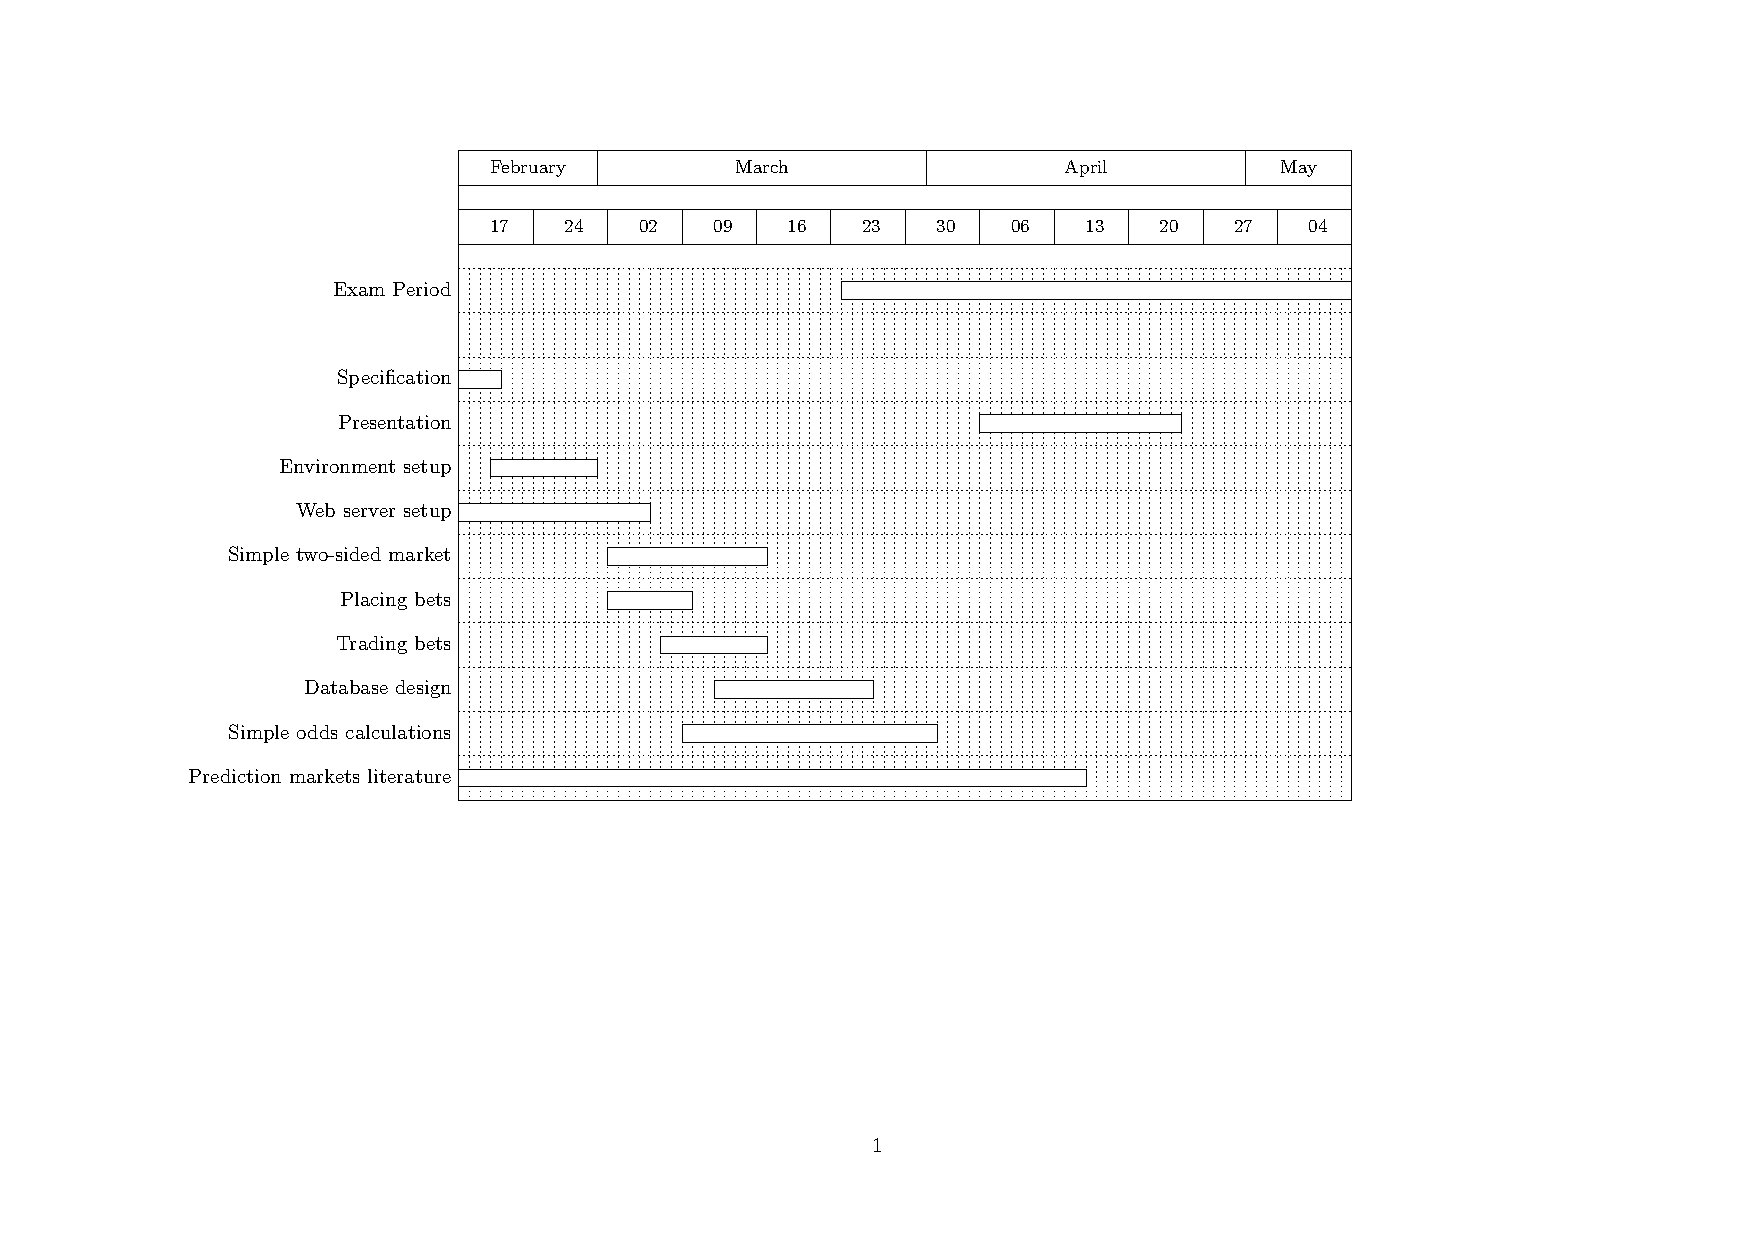
\includepdf[landscape=true,pages=1,pagecommand={\section{Timetable}, \label{app:timetable}}]{timetable.pdf}
    \includepdf[landscape=true,pages=2,pagecommand={}]{timetable.pdf}

\end{appendices}

\end{document}
